\documentclass[tikz]{standalone}
\usepackage{tikz}
\usepackage{circuitikz}

\begin{document}
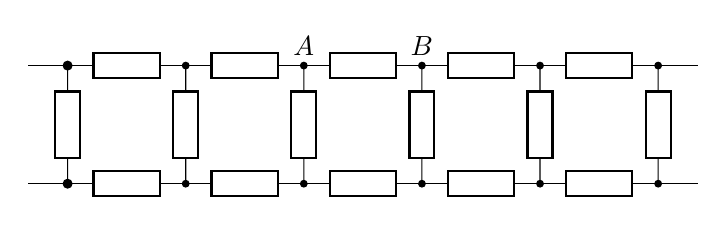
\begin{tikzpicture}[european]
	\draw (0,0) to [short, -*] (0.5,0) to [R, -*, /tikz/circuitikz/bipoles/length=30pt] (2,0) to [R, -*, /tikz/circuitikz/bipoles/length=30pt] (3.5,0) to [R, -*, /tikz/circuitikz/bipoles/length=30pt] (5,0) to [R, -*, /tikz/circuitikz/bipoles/length=30pt] (6.5,0) to [R, -*, /tikz/circuitikz/bipoles/length=30pt] (8,0) to [short, -] (8.5,0);
	\draw (0,1.5) to [short, -*] (0.5,1.5) to [R, -*, /tikz/circuitikz/bipoles/length=30pt] (2,1.5) to [R, -*, /tikz/circuitikz/bipoles/length=30pt] (3.5,1.5) node [above] {$A$} to [R, -*, /tikz/circuitikz/bipoles/length=30pt] (5,1.5) node [above] {$B$} to [R, -*, /tikz/circuitikz/bipoles/length=30pt] (6.5,1.5) to [R, -*, /tikz/circuitikz/bipoles/length=30pt] (8,1.5) to [short, -] (8.5,1.5);
	\draw (0.5,0) to [R, /tikz/circuitikz/bipoles/length=30pt] (0.5,1.5) (2,0) to [R, /tikz/circuitikz/bipoles/length=30pt] (2,1.5) (3.5,0) to [R, /tikz/circuitikz/bipoles/length=30pt] (3.5, 1.5) (5,0) to [R, /tikz/circuitikz/bipoles/length=30pt] (5, 1.5) (6.5,0) to [R, /tikz/circuitikz/bipoles/length=30pt] (6.5, 1.5) (8,0) to [R, /tikz/circuitikz/bipoles/length=30pt] (8,1.5);
\end{tikzpicture}
\end{document}
